% This is based on "sig-alternate.tex" V1.9 April 2009
% This file should be compiled with V2.4 of "sig-alternate.cls" April 2009
%
\documentclass{report}

\usepackage[english]{babel}
\usepackage{graphicx}
\usepackage{tabularx}
\usepackage{subfigure}
\usepackage{enumitem}
\usepackage{url}


\usepackage{color}
\definecolor{orange}{rgb}{1,0.5,0}
\definecolor{lightgray}{rgb}{.9,.9,.9}
\definecolor{java_keyword}{rgb}{0.37, 0.08, 0.25}
\definecolor{java_string}{rgb}{0.06, 0.10, 0.98}
\definecolor{java_comment}{rgb}{0.12, 0.38, 0.18}
\definecolor{java_doc}{rgb}{0.25,0.35,0.75}

% code listings

\usepackage{listings}
\lstloadlanguages{Java}
\lstset{
	language=Java,
	basicstyle=\scriptsize\ttfamily,
	backgroundcolor=\color{lightgray},
	keywordstyle=\color{java_keyword}\bfseries,
	stringstyle=\color{java_string},
	commentstyle=\color{java_comment},
	morecomment=[s][\color{java_doc}]{/**}{*/},
	tabsize=2,
	showtabs=false,
	extendedchars=true,
	showstringspaces=false,
	showspaces=false,
	breaklines=true,
	numbers=left,
	numberstyle=\tiny,
	numbersep=6pt,
	xleftmargin=3pt,
	xrightmargin=3pt,
	framexleftmargin=3pt,
	framexrightmargin=3pt,
	captionpos=b
}

% Disable single lines at the start of a paragraph (Schusterjungen)

\clubpenalty = 10000

% Disable single lines at the end of a paragraph (Hurenkinder)

\widowpenalty = 10000
\displaywidowpenalty = 10000
 
% allows for colored, easy-to-find todos

\newcommand{\todo}[1]{\textsf{\textbf{\textcolor{orange}{[[#1]]}}}}

% consistent references: use these instead of \label and \ref

\newcommand{\lsec}[1]{\label{sec:#1}}
\newcommand{\lssec}[1]{\label{ssec:#1}}
\newcommand{\lfig}[1]{\label{fig:#1}}
\newcommand{\ltab}[1]{\label{tab:#1}}
\newcommand{\rsec}[1]{Section~\ref{sec:#1}}
\newcommand{\rssec}[1]{Section~\ref{ssec:#1}}
\newcommand{\rfig}[1]{Figure~\ref{fig:#1}}
\newcommand{\rtab}[1]{Table~\ref{tab:#1}}
\newcommand{\rlst}[1]{Listing~\ref{#1}}



%%% Our own commands
\newcommand{\name}{Shopping XYZ }
\usepackage{verbatim}
\graphicspath{ {img/} }


\usepackage{hyperref}
%\usepackage[nameinlink,noabbrev]{cleveref}

% General information

\title{\name\\
\normalsize{Distributed Systems -- Project Proposal}}
\subtitle{subtitle}

% Use the \alignauthor commands to handle the names
% and affiliations for an 'aesthetic maximum' of six authors.

\numberofauthors{1} %  in this sample file, there are a *total*
% of EIGHT authors. SIX appear on the 'first-page' (for formatting
% reasons) and the remaining two appear in the \additionalauthors section.
%
\author{
% You can go ahead and credit any number of authors here,
% e.g. one 'row of three' or two rows (consisting of one row of three
% and a second row of one, two or three).
%
% The command \alignauthor (no curly braces needed) should
% precede each author name, affiliation/snail-mail address and
% e-mail address. Additionally, tag each line of
% affiliation/address with \affaddr, and tag the
% e-mail address with \email.
%
% 1st. author
	\alignauthor \normalsize{IVANOV Danil, SANSONETTI Luigi, H�NER Dominik, DRESCHER Lukas}\\
		\affaddr{\normalsize{ETH ID 1: 15-826-415,
		ETH ID 2: 14-803-688,
		ETH ID 3: 14-945-133
		ETH ID 4: XX-XXX-XXX}}\\
		\email{\normalsize{divanov@student.ethz.ch,
		sluigi@student.ethz.ch,
		dhaener@student.ethz.ch,
		lukasd@student.ethz.ch}}
}


\begin{document}

\maketitle

	\begin{abstract}
		As of today, there is no open-source Android application that solves the consensus
		problem in a flat-share situation. As a result, users too often have to juggle
		between apps, trying to manually maintain an updated state of the situation on
		several different phones.
	
		\name is an Android application to streamline the efficiency of grocery acquisition
		in a shared living accommodation. The main idea is to implement a platform for devices to
		communicate without the use of a centralised server. Using the concepts of distributed
		computing, \name maintains an updated state of various lists across all devices 
		in a cluster.
	
		\begin{description}
			\item[System overview:] 
				Implementation will be decentralised and distributed among
				the users. Each node will act as a client and a server, supplying
				the rest of the cluster with the required information for maintaining
				consensus.
			\item[Software and hardware used in this project:] 
				The application will be implemented on Android phones, using the Android SDK
				in conjunction with Java.
				The application requires internal storage, as well as internet access.
			\item[Expected deliveries:]
				An Android application that solves the aforementioned problem, using
				distributed computing concepts.
		\end{description}
		
		\name provides a very extensible platform, such ideas include: \begin{itemize}
			\item An event organiser
			\item A debt/expense tracking system
			\item A meal planner
		\end{itemize}
	\end{abstract}

	\section{Introduction}

	Manually updating a shared shopping list is an error-prone process that doesn't scale.
	The task constitutes a high cognitive load for humans, leading to mistakes and oversights during
	manual maintenance of the said list.
	
	\name maintains the state of a shopping list distributed across several devices without relying
	on a central server. \\
	
	However, by distributing this task, the consensus problem is to be taken into account ; it is
	important to make sure that all nodes agree upon the information, and to make sure that every change
	is communicated.
	
	Each node implements a client/server architecture. The client listens to other servers for updates.
	The server communicates changes to other clients.
	
	In order to maintain consensus over the shared list, a node notifies other when it modifies the list,
	and makes that all other nodes acknowledge the change. Upon connection to the network, the new node
	queries for the latest version of the said list.
	
	Furthermore, not having a central server to rely on raises the question of how to create a closed network.
	
	To build this platform, the following technological problem must be solved : 
	"How to implement a distributed communication system over a network of Android devices ?"

	\section{System Overview}

		\begin{description}
			\item[Technical plan:]
				\name requires the implementation of a distributed client/server logic 
				among a network of android devices as well as the development of a UI design. \\
				
				Any device can invite another one to its flat-share (network) by sending it an invite.
				The new device, upon entering the network, gets the set of all IP addresses of the other
				nodes, and broadcasts its own IP address to them. Every device keeps a set of the IP addresses
				of all the nodes in their network.
				
				The application contains a service that would check whether the devices IP address changed.
				If it did, the application immediately broadcast its new address to the network, and all other
				nodes will update their IP addresses sets. \\
				
				Upon performing a legal operation on an element in any list, the node responsible
				of this manipulation will immediately notify all other nodes of this manipulation.
				
			\item[UI design:] The user interface will be similar to the following:
			
				\begin{figure}[h]
					\centering
   					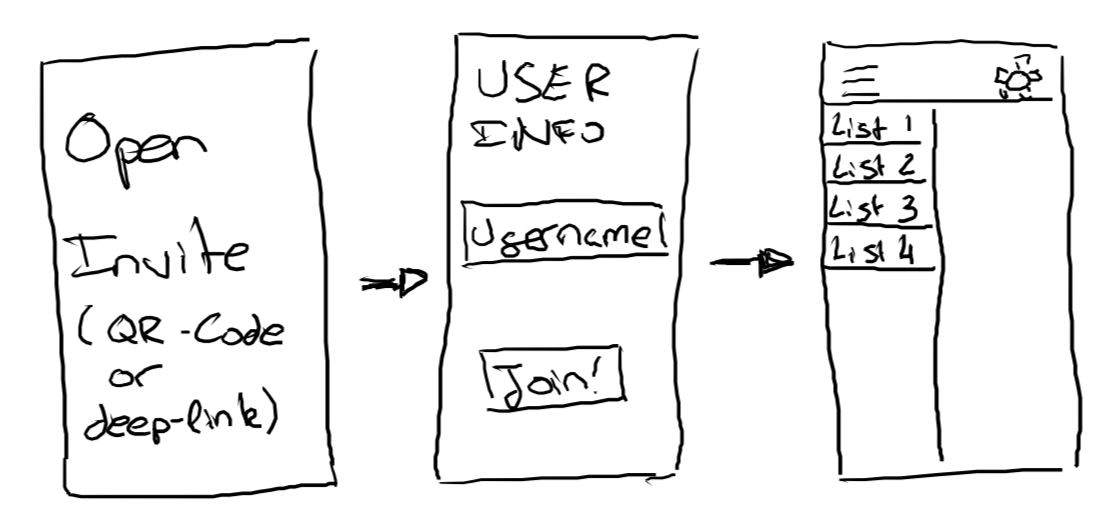
\includegraphics[width=\columnwidth]{UI.png}
					\caption{UI sketch}
				\end{figure}
				
			\item[Communication design:]
			
				The communication relies on a peer-to-peer architecture.
				
				The protocol to join a network is as follows:
				
				\begin{figure}[h!]
					\centering
   					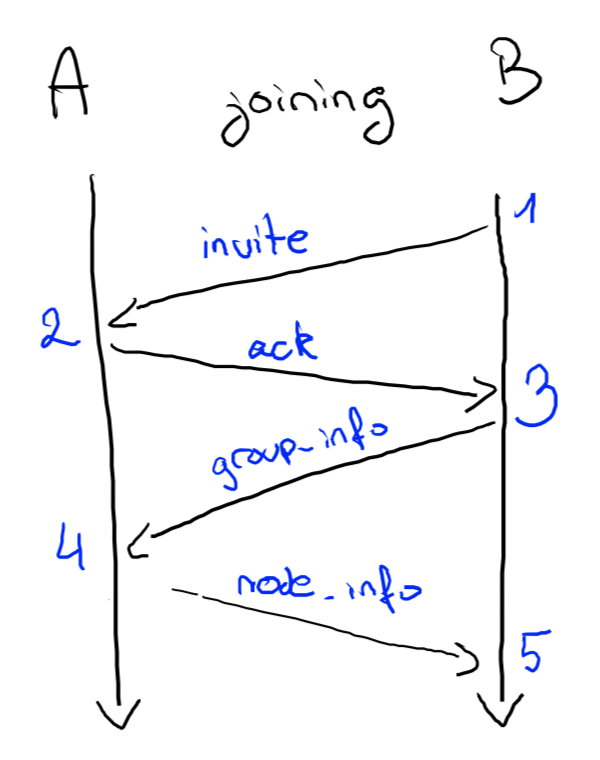
\includegraphics[width=\columnwidth]{protocol.png}
					\caption{Joining protocol timeline}
					\label{fig:joiningProtocol}
				\end{figure}
				
				\begin{enumerate}
					\item Node B sends an invite to node A via an external channel 
						(messaging service or QR-code).
					\item Node A acknowledges the invitation and sends its IP to B.
					\item Node B sends the set of the IP addresses and their corresponding IDs
						of every node in the network.
					\item Node A broadcasts its IP and ID to all the nodes in the network.
					\item Every node updates their IP/ID map with the new entry.
				\end{enumerate}
				
				(See \autoref{fig:joiningProtocol})
				
				Upon joining a network, a node A accesses the public list, which is shared between every node,
				and creates
				\begin{itemize}
					\item a personal private list that will be known only to A,
					\item a personal public list that will be known to every node in the network.
				\end{itemize}
				
				Suppose node A is trying to reconnect to the network. The protocol is as follows:
				\begin{enumerate}
					\item A broadcasts a reconnection request message to all the nodes in the network.
					\item Every node getting this message acknowledges it.
					\item Let B be the first node to acknowledge A's message. 
						A queries B for its set of IPs and IDs.
					\item A updates its set of IPs and IDs, and broadcasts it.
				\end{enumerate}
				
				In the case where every node is disconnected (i.e.: A gets no acknowledgement message to
				its reconnection request), the network has to be created again. The joining protocol is
				therefore repeated for all the disconnected nodes when they reconnect in a way that will
				save the existing data.
				
			\item[Application design:]
				When a node A tries to apply a modification with a parameter to an item of a list,
				it simply broadcasts the following message:
				\begin{figure}[h!]
					\begin{tabular}{|c|c|c|c|c|c|}
						\hline
							A's ID & list & modif. & value & item ID & previous value \\
						\hline
					\end{tabular}
					\centering
					\caption{Modification message content}
				\end{figure} \\
				where the item ID is the hash of the item's value.
				
				The modification can be either "add", "remove", "update", "makePublic" or "makePrivate".
				\begin{itemize}
					\item Add: takes a list ID L, a value V and an ID I as parameters, and adds the item
						of ID I and value V to L.
					\item Remove: takes a list ID L and an ID I as parameters, and removes the item of
						ID I of the list L.
					\item Update: Takes a list ID L, a value V and an ID I as parameters, and updates
						the value of the element of ID I of list L to V.
					\item makePublic: Takes an ID I, removes the element of ID I of the node's 
						personal private list, and adds it to the node's personal public list.
					\item makePrivate: Takes an ID I, removes the element of ID I of the node's 
						personal public list, and adds it to the node's personal private list.
				\end{itemize}
		
			\item[Expected issues:] All nodes disconnecting from the network would require the network to be
				rebuilt. This problem is rather minor, given that \begin{enumerate}[label=\alph*)]
					\item In small networks, rebuilding is fast,
					\item The larger the network, the greater the chances of at least one node being connected.
				\end{enumerate}
				
				If two nodes propose changes at the same time, then the following happens: \begin{itemize}
					\item Add and Update: The user is asked to resolve the conflict manually.
					\item Remove: The item is simply removed.
					\item makePublic and makePrivate: only the node in question can perform those operations
						on its lists.
				\end{itemize}
				
				\begin{figure}[h!]
					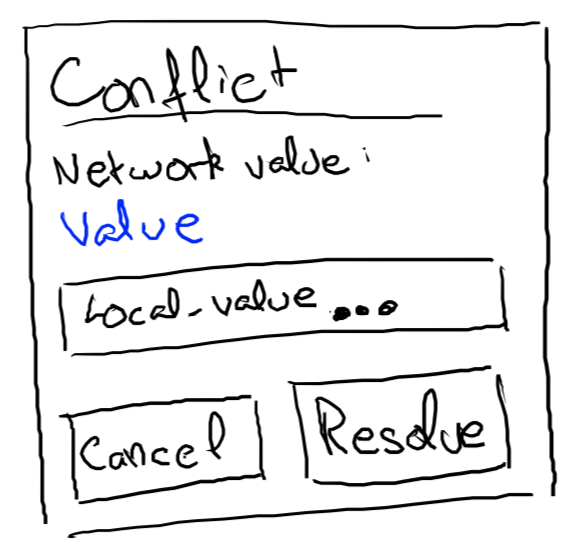
\includegraphics[width=\columnwidth]{conflict.png}
					\centering
					\caption{Conflict solving prompt}
					\label{fig:conflict}
				\end{figure}
				
				\autoref{fig:conflict} shows what the user will be prompted to solve a conflict.
				The user can modify the \textit{local\_value} text field to resolve the conflict, or cancel to
				accept the network value.
				
		\end{description}		

	\section{Requirements}
		
		A basic Android phone with internet connectivity is required.
		
		Given that several lists will be stored on every device, some storage space is required as well (a few MB).

	\section{Work Packages}
	
		Breakdown of the work to subtasks to meet the project requirements.

		\begin{description} 
        	\item[Joining protocol:] Implement the protocol for a node to join a network.
			\item[Communication protocol:] Implement the protocol to allow nodes to communicate.
			\item[List manipulation:] Implement list logic (modification operations, UI communication).
        	\item[UI design:] Implement UI design.
			\item[Presentation:] Prepare the presentation slides, project logo, and demo.
		\end{description}

	\section{Milestones}

		\subsection{Division of tasks}
		
			\begin{description} 
        		\item[Joining protocol:] Danil, Luigi.
				\item[Communication protocol:] Lukas, Dominik.
				\item[List manipulation:] Danil, Luigi.
       		 	\item[UI design:] Lukas, Dominik.
				\item[Presentation:] Everybody.
			\end{description}
		
		\subsection{Schedule}
		
			\begin{description}
				\item[26/11:] Joining protocol implemented. 
				\item[03/12:] Communication protocol and list logic implemented.
				\item[10/12:] UI design implemented.
				\item[15/12:] Presentation and logo ready.
				\item[17/12:] Project completed, functioning demo.
			\end{description}

	\section{References}
	
		\begin{enumerate}
			\item Computer Networking: A Top-Down Approach, 6th Edition, 
				James F. Kurose, University of Massachusetts, Amherst, 
				Keith W. Ross, Polytechnic University, Brooklyn.
			\item EPFL's COM-208 (Computer Networks), Katerina Argyraki
		\end{enumerate}

	% The following two commands are all you need in the
	% initial runs of your .tex file to
	% produce the bibliography for the citations in your paper.
	\bibliographystyle{abbrv}
	\bibliography{report}

\end{document}
